\documentclass[noinstructornotes]{ximera}
%handout:  for handout version with no solutions or instructor notes
%handout,instructornotes:  for instructor version with just problems and notes, no solutions
%noinstructornotes:  shows only problem and solutions

%% handout
%% space
%% newpage
%% numbers
%% nooutcomes

%I added the commands here so that I would't have to keep looking them up
%\newcommand{\RR}{\mathbb R}
%\renewcommand{\d}{\,d}
%\newcommand{\dd}[2][]{\frac{d #1}{d #2}}
%\renewcommand{\l}{\ell}
%\newcommand{\ddx}{\frac{d}{dx}}
%\everymath{\displaystyle}
%\newcommand{\dfn}{\textbf}
%\newcommand{\eval}[1]{\bigg[ #1 \bigg]}

%\begin{image}
%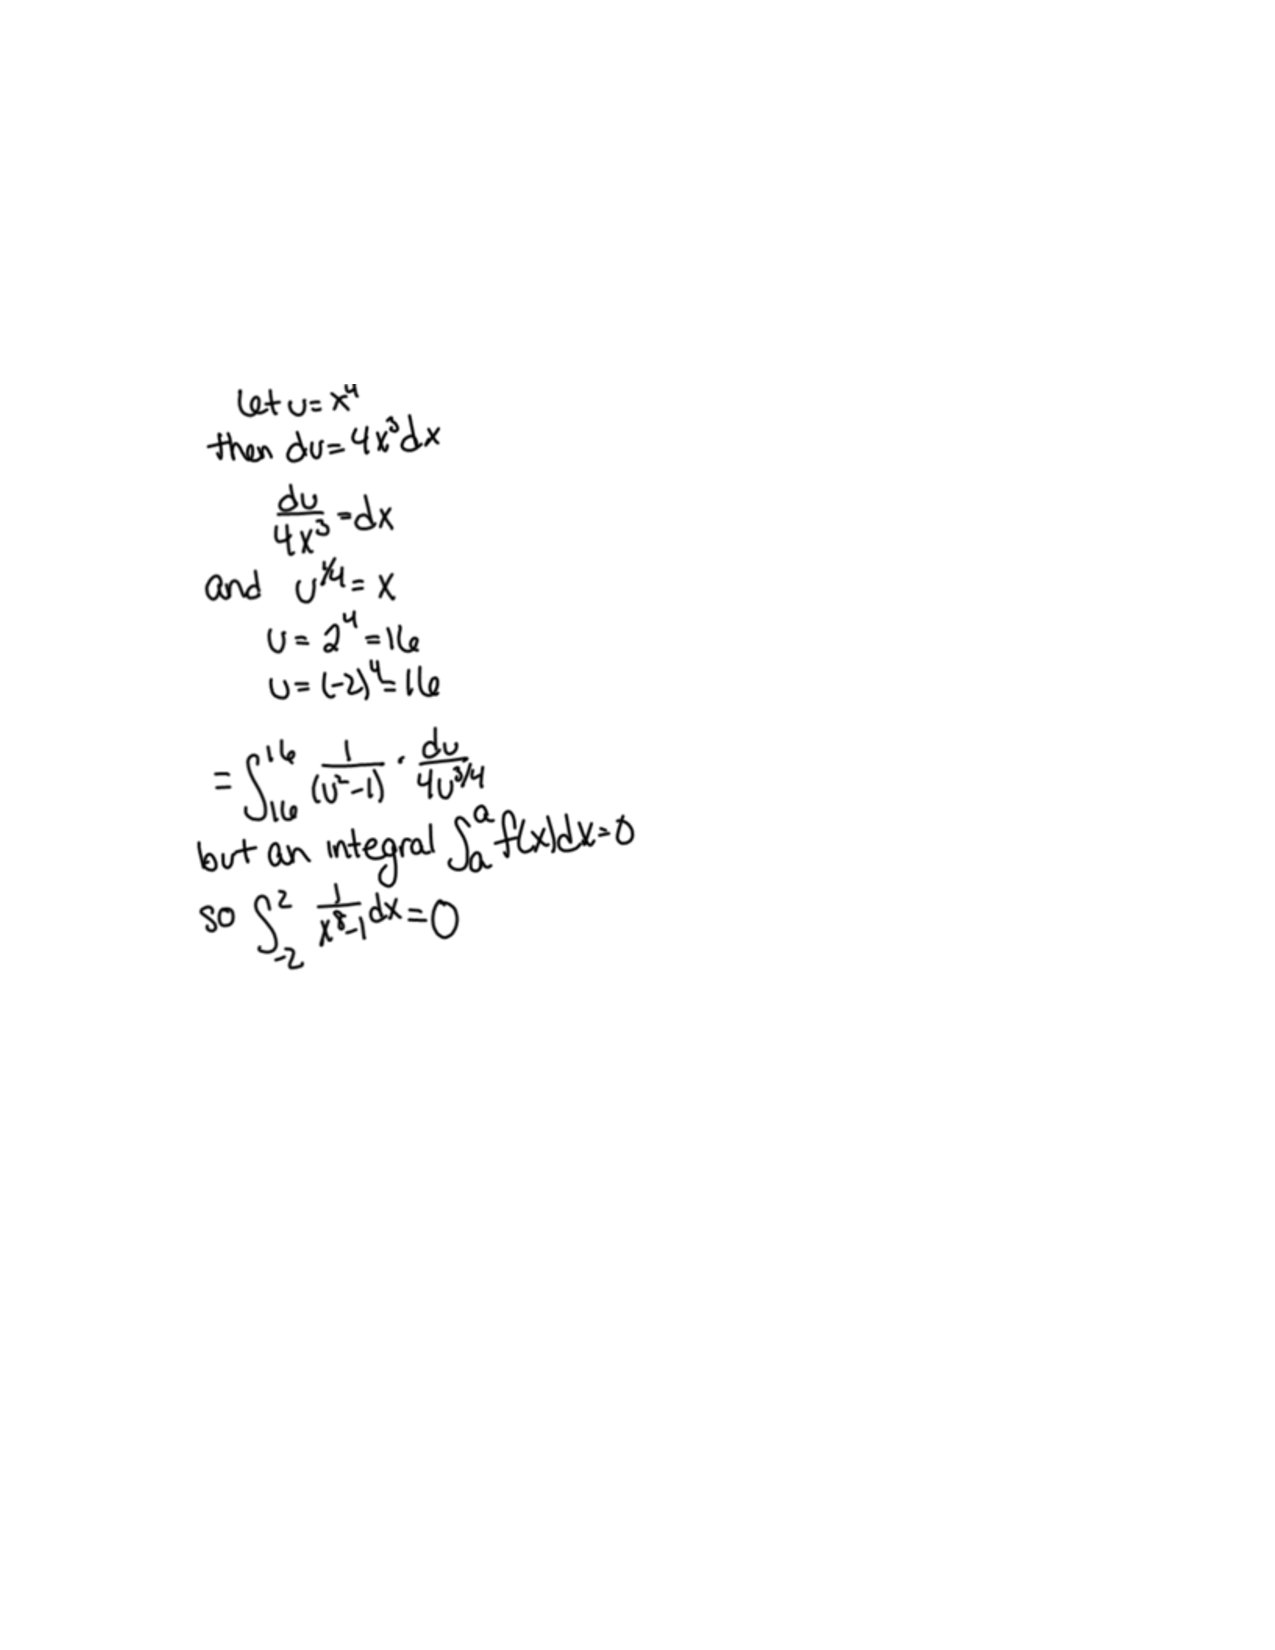
\includegraphics[trim= 170 420 250 180]{Figure1.pdf}
%\end{image}

%add a ``.'' below when used in a specific directory.
\newcommand{\RR}{\mathbb R}
\renewcommand{\d}{\,d}
\newcommand{\dd}[2][]{\frac{d #1}{d #2}}
\renewcommand{\l}{\ell}
\newcommand{\ddx}{\frac{d}{dx}}
\newcommand{\dfn}{\textbf}
\newcommand{\eval}[1]{\bigg[ #1 \bigg]}

\usepackage{multicol}

\renewenvironment{freeResponse}{
\ifhandout\setbox0\vbox\bgroup\else
\begin{trivlist}\item[\hskip \labelsep\bfseries Solution:\hspace{2ex}]
\fi}
{\ifhandout\egroup\else
\end{trivlist}
\fi} %% we can turn off input when making a master document

\title{Recitation \# 2 Regions Between Curves - Solutions}  

\begin{document}
\begin{abstract}		\end{abstract}
\maketitle


%There was not a warm-up exercise for this specific section
\begin{comment}
\section{Warm up:}

	\begin{freeResponse}
	
	\end{freeResponse}
	
\begin{instructorNotes}

\end{instructorNotes}
\end{comment}







\section{Group work:}



%problem 1
\begin{problem}
Consider the region bounded by the curves $y=2x^2-7x+8$ and $y=x^2-4x+18$.
	\begin{enumerate}
		\item  Draw a sketch of the graphs.
		\begin{freeResponse}
			\begin{image}
			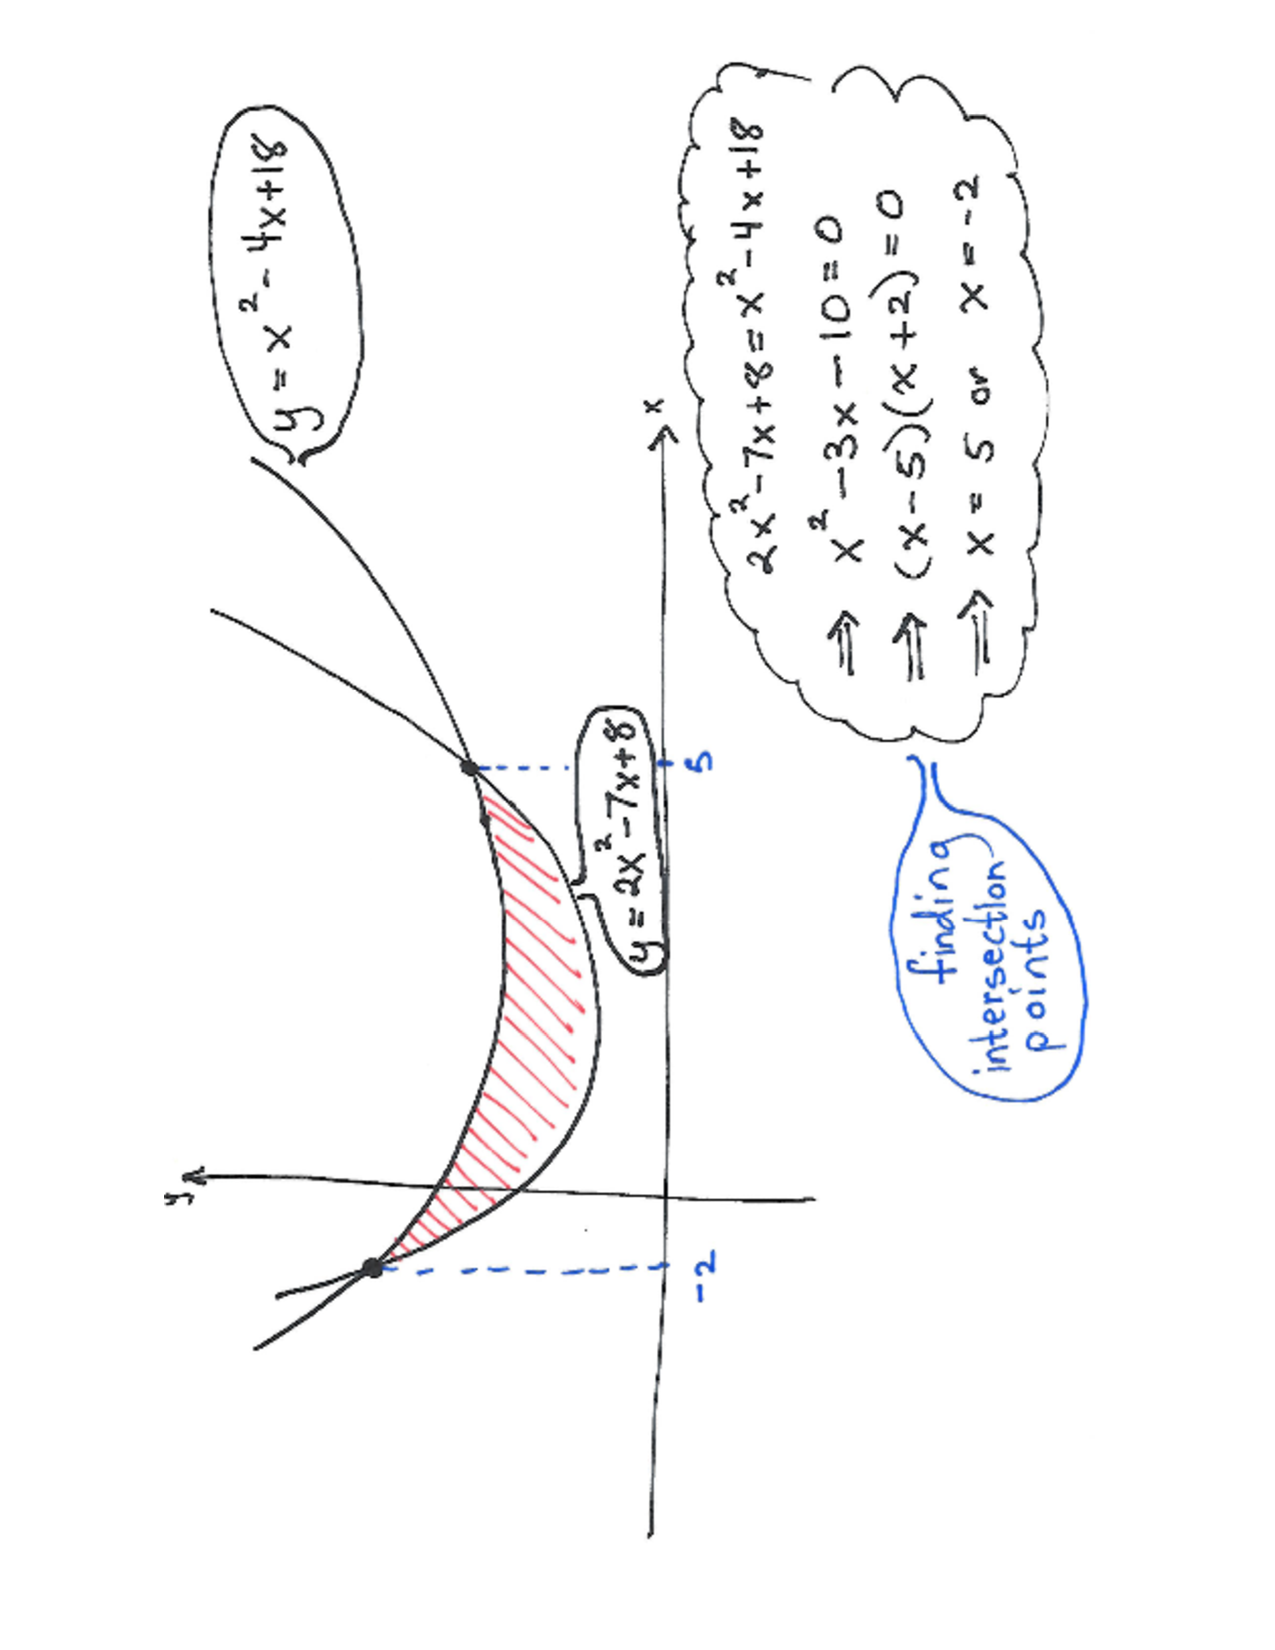
\includegraphics[trim= 50 320 50 180,scale=0.6,angle=-89.99]{Figure6-2-2.pdf}
			\end{image}
		\end{freeResponse}
		
		\item  Find the area between these curves.
		\begin{freeResponse}
		Let $y_1 = 2x^2-7x+8$ and $y_2=x^2-4x+18$.  
		By the solution to part (a), we know both that $y_1 - y_2 = x^2 - 3x - 10$ and that these two curves intersect at $x=-2, 5$.  
		By checking the point $x=0$ (or by looking at the graph from part (a)) we see that $y_2 \geq y_1$ on the interval $[-2,5]$.  
		So the area between the curves is:
			\begin{align*}
			\int_{-2}^5 (y_2 - y_1) \d x &= \int_{-2}^5 (-x^2 + 3x + 10) \d x  \\
			&= \eval{-\frac{1}{3} x^3 + \frac{3}{2} x^2 + 10x}_{-2}^5  \\
			&= \left(- \frac{125}{3} + \frac{75}{2} + 50 \right) - \left( \frac{8}{3} + 6 - 20 \right)  \\
			&= - \frac{133}{3} + \frac{75}{2} + 64  \\
			&= \frac{-266 + 225 + 384}{6} = \frac{343}{6}
			\end{align*}
		\end{freeResponse}
		
		\item  Find the area of the region bounded by the curves $x=2y^2-7y+8$ and $x=y^2-4y+18$.
		\begin{freeResponse}
		This region is exactly the same as the {\color{red} red region} from part (a), except it is rotated clockwise by $90^{\circ}$.  
		Since the area of a region does not change under rotation, we have that the area of the new region is still $\frac{343}{6}$.  
		\end{freeResponse}
		
		\item  Find the area of the region bounded by the curves
			\begin{enumerate}
				\item[(i)]  $y = 2x^2 - 7x$ and $y=x^2 - 4x + 10$.
				\begin{freeResponse}
				The region bounded by the curves $y = 2x^2 - 7x$ and $y=x^2 - 4x + 10$ is just the {\color{red} red region} in part (a) translated downward by 8 units.  
				Since the area of a region does not change under translation, we have that the area of the new region is still $\frac{343}{6}$.  
				\end{freeResponse}
				
				\item[(ii)]  $y=2x^2-7x-30$ and $y=x^2-4x-20$.
				\begin{freeResponse}
				This is the same as (i), except now the {\color{red} red region} has been translated downward by 38 units.  
				Therefore, the area of this region is still $\frac{343}{6}$.  
				\end{freeResponse}
				
			\end{enumerate}
		
		\item  Find the area of the region bounded by the curves $y=2x^2-7x+8$, $y=x^2-4x+18$, $x=1$, and $x=6$.
		\begin{freeResponse}
			\begin{image}
			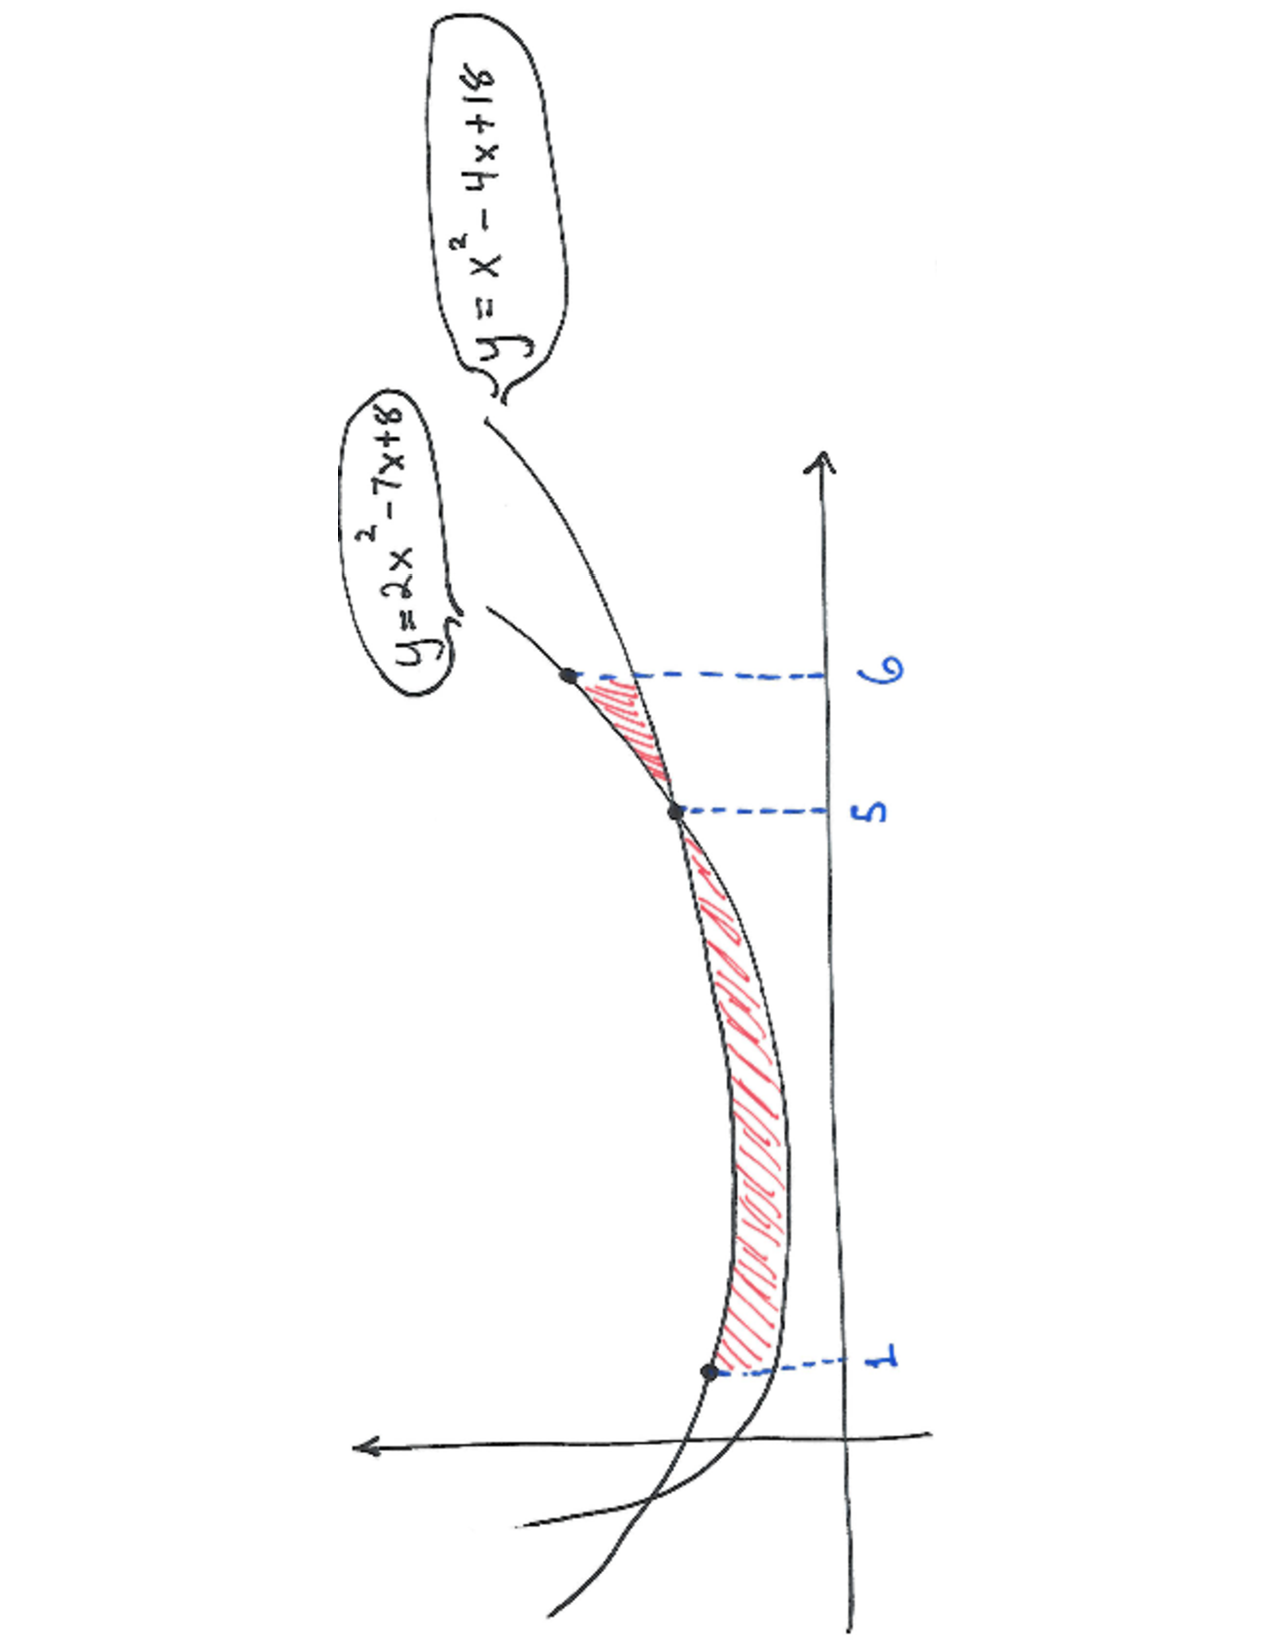
\includegraphics[trim= 120 250 130 180,scale=0.6,angle=-89.99]{Figure6-2-3.pdf}
			\end{image}
		We already know that the graphs of the two functions intersect at the point $x=5$.  
		By checking the points $x=1$ and $x=6$ (or by looking at the graph above) we see that 
			\begin{align*}
			y_2 \geq y_1 \quad \text{on} \quad [1,5]  \\
			y_1 \geq y_2 \quad \text{on} \quad [5,6]
			\end{align*}
		Thus, the area between the curves is
			\begin{align*}
			&\int_1^5 (y_2 - y_1) \d x + \int_5^6 (y_1 - y_2) \d x  \\
			&= \int_1^5 (-x^2 + 3x + 10) \d x + \int_5^6 (x^2 - 3x - 10) \d x  \\
			&= \eval{-\frac{1}{3} x^3 + \frac{3}{2} x^2 + 10x}_1^5 + \eval{\frac{1}{3} x^3 - \frac{3}{2} x^2 - 10x}_5^6  \\
			&= \left[ \left(- \frac{125}{3} + \frac{75}{2} + 50 \right) - \left( - \frac{1}{3} + \frac{3}{2} + 10 \right) \right] + \left[ \left( 72 - 54 - 60 \right) - \left( \frac{125}{3} - \frac{75}{2} - 50 \right) \right]  \\
			&= - \frac{249}{3} + \frac{147}{2} + 48  = -83 + 48 + \frac{147}{2} = \frac{-70 + 147}{2} = \frac{77}{2}  
			\end{align*}
		\end{freeResponse}
		
	\end{enumerate}
	
\end{problem}

\begin{instructorNotes}
Have the students do (a) and (b), and then have a group present.  
Afterwards, discuss the variations (c) and (d) as a whole class.
\end{instructorNotes}







%problem 2
\begin{problem}
Set up a single integral that computes the area of the region bounded by the curves (and be sure to draw a sketch of the graphs).
	\begin{enumerate}
		\item  $x=y^2$ and $y=6-x$
		\begin{freeResponse}
			\begin{image}
			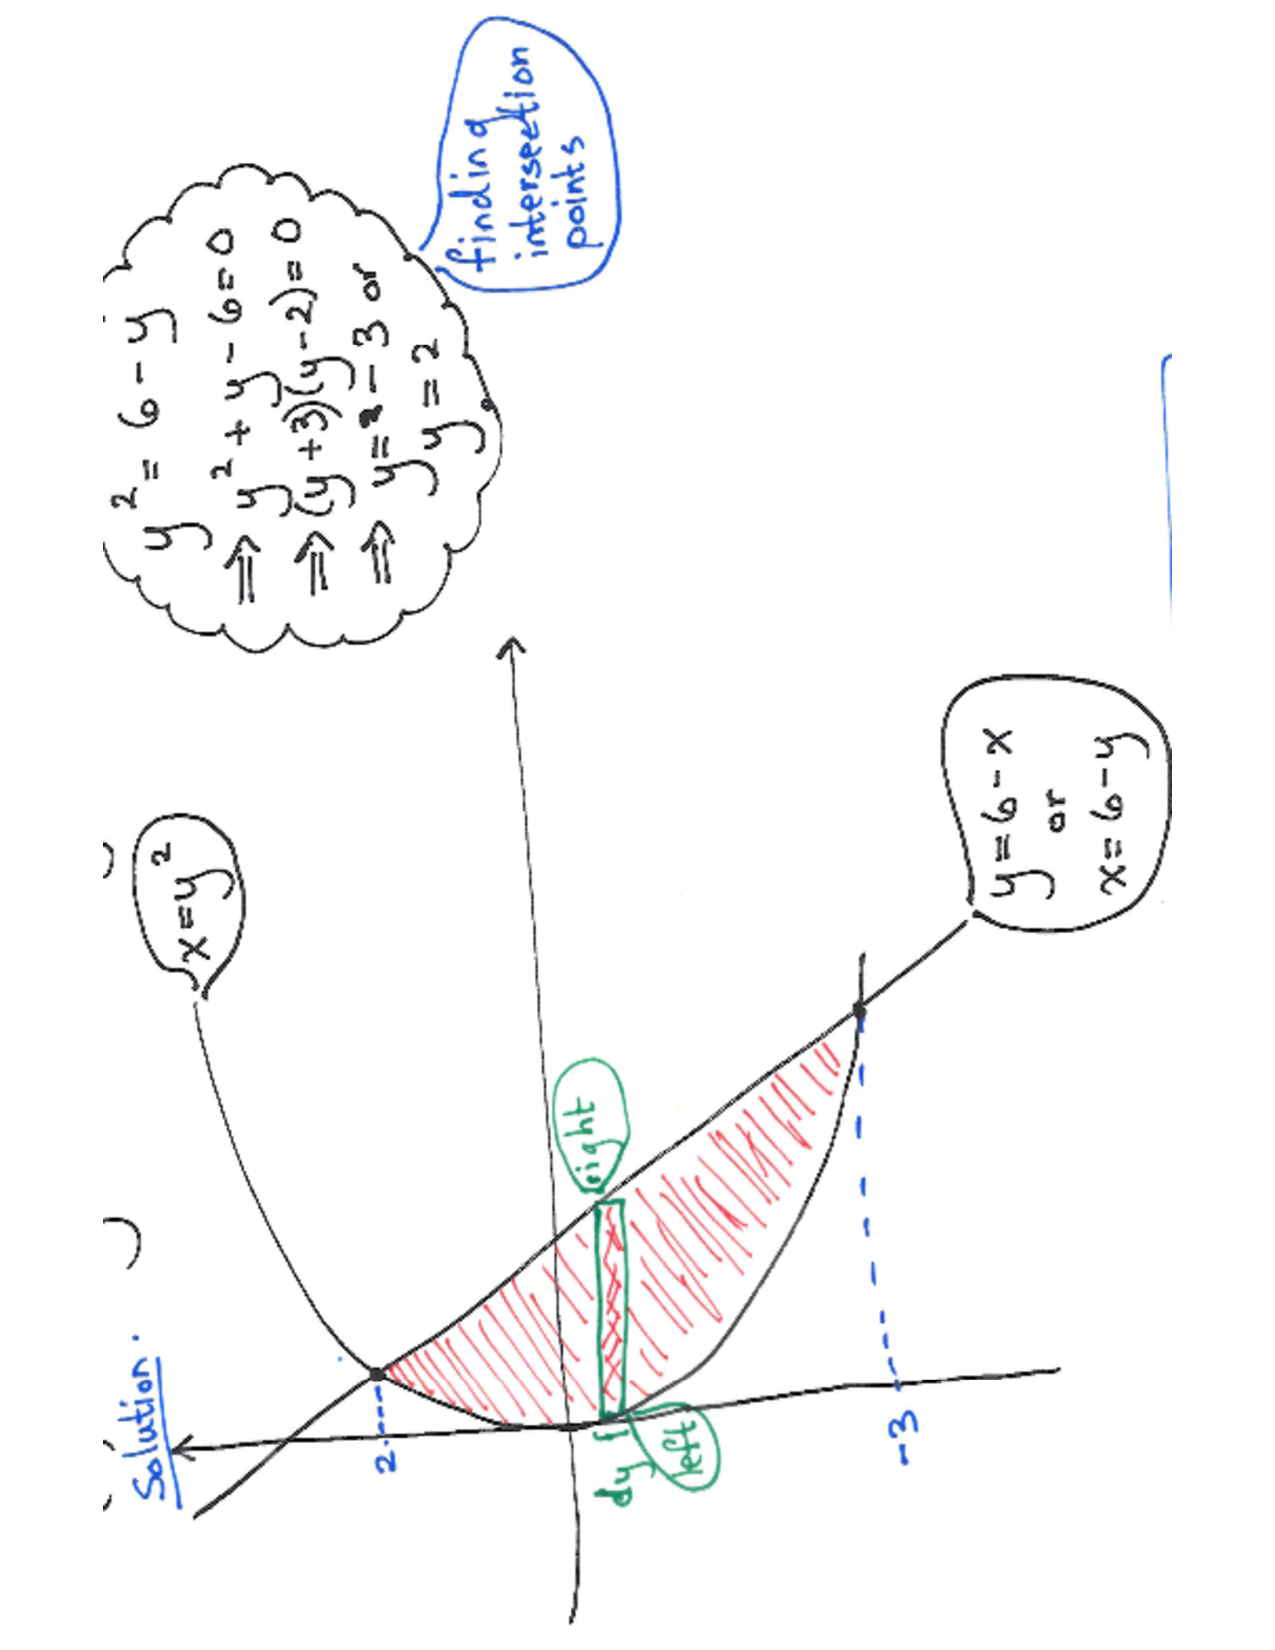
\includegraphics[trim= 30 270 50 180,scale=0.6,angle=-89.99]{Figure6-2-4.pdf}
			\end{image}
		Thus,
		\[
		\text{{\color{red} Area of region}} =  \int_{-3}^2 [(6-y) - y^2] \d y .
		\]
		\end{freeResponse}
		
		\item  $y=x^2 + 6$ and $y=3x+10$
		\begin{freeResponse}
			\begin{image}
			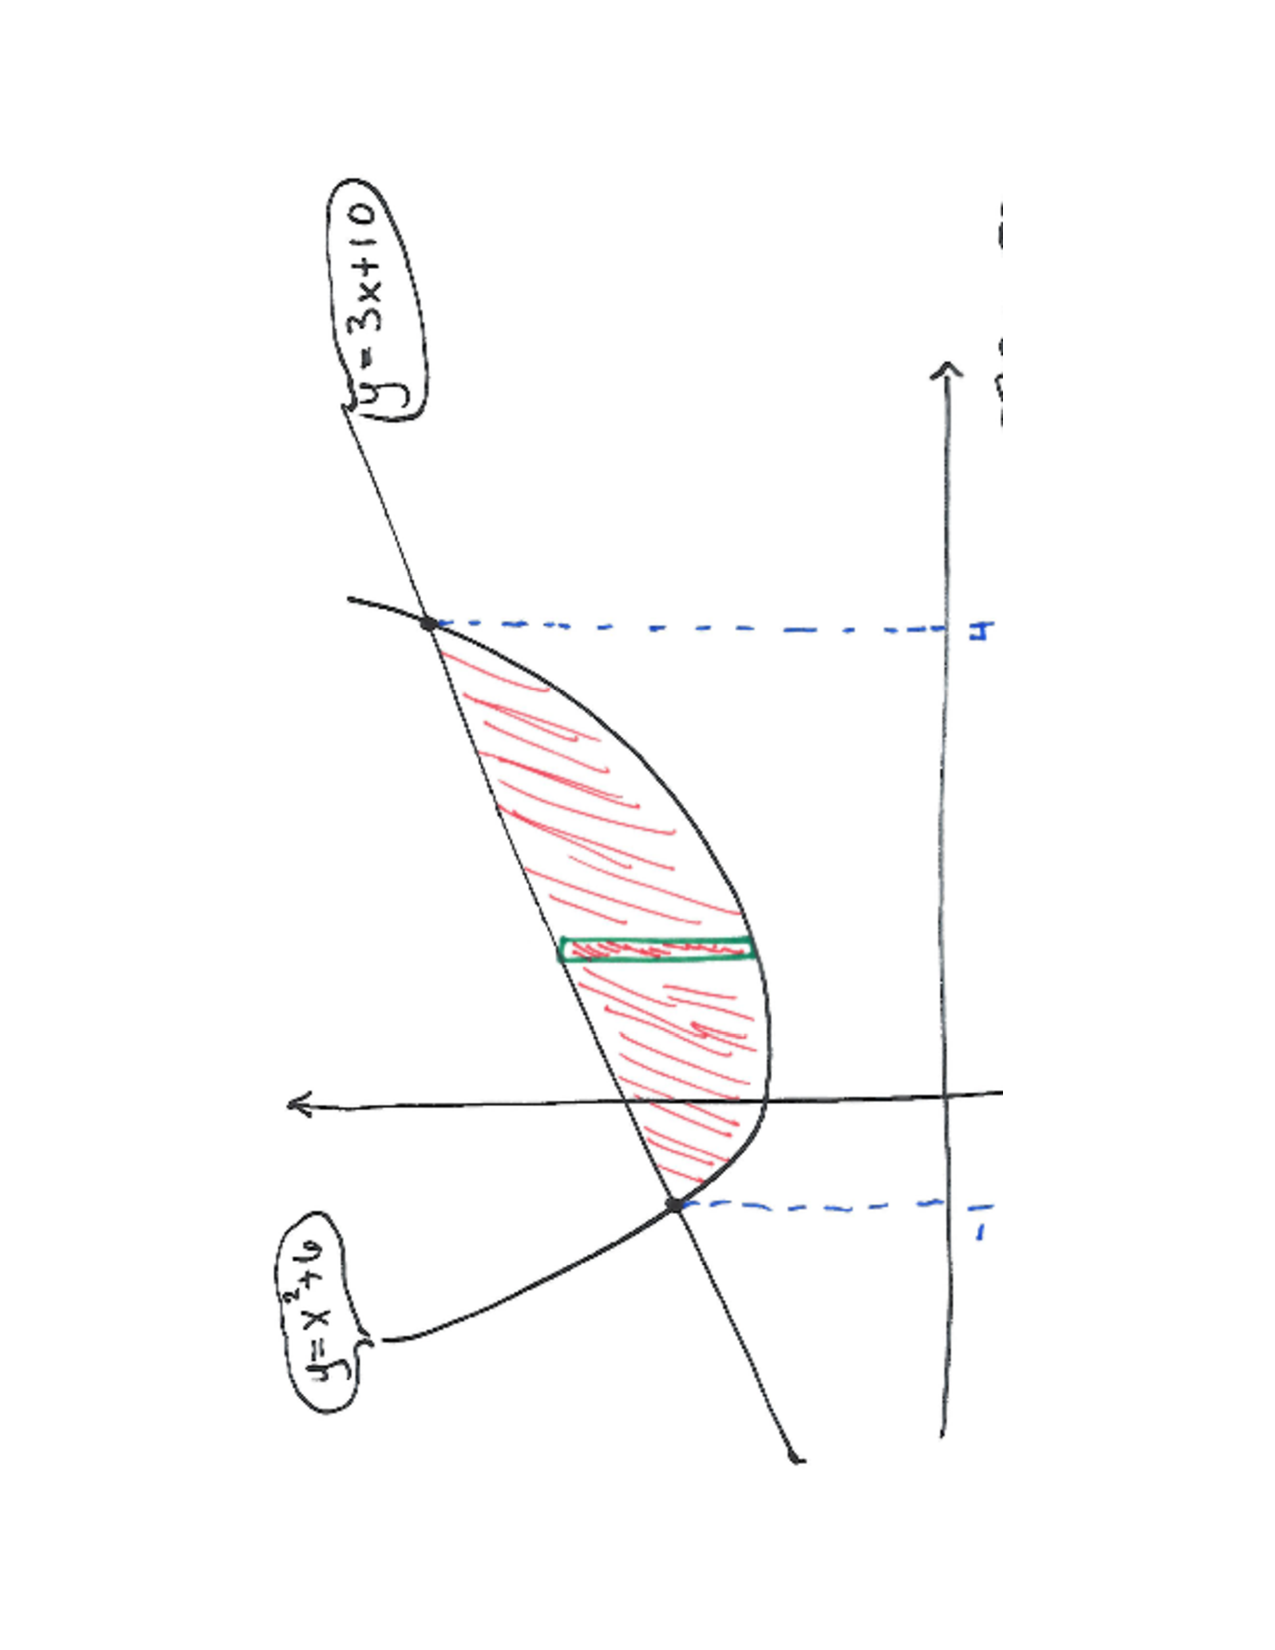
\includegraphics[trim= 100 270 100 180,scale=0.6,angle=-89.99]{Figure6-2-5.pdf}
			\end{image}
		To find the intersection points in the above picture, we solve
			\begin{align*}
			x^2 + 6 &= 3x + 10  \\
			x^2 - 3x - 4 &= 0  \\
			(x+1)(x-4) &= 0  \\
			x &= -1, 4.
			\end{align*}
		So
		\[
		\text{{\color{red} Area of region}} =  \int_{-1}^4 [(3x+100) - (x^2 + 6)] \d x .
		\]
		\end{freeResponse}
		
	\end{enumerate}

\end{problem}

\begin{instructorNotes}
Split (a) and (b) among the groups.  
Note that (a) should be set up in terms of $y$ while (b) should be set up in terms of $x$.  
Have groups present their solutions.  
Discuss with the students factors to consider when deciding whether to integrate in terms of $x$ or $y$.
\end{instructorNotes}







%problem 3
\begin{problem}
Two runners ($A$ and $B$) run in a race in which the winner runs the farthest in $4$ minutes.  
The runners' respective velocities are
\[
v_A(t) = \frac{1}{3} t^2	\qquad	 v_B(t) = t
\]
The graphs of the runners' velocities is given below.  

\begin{image}
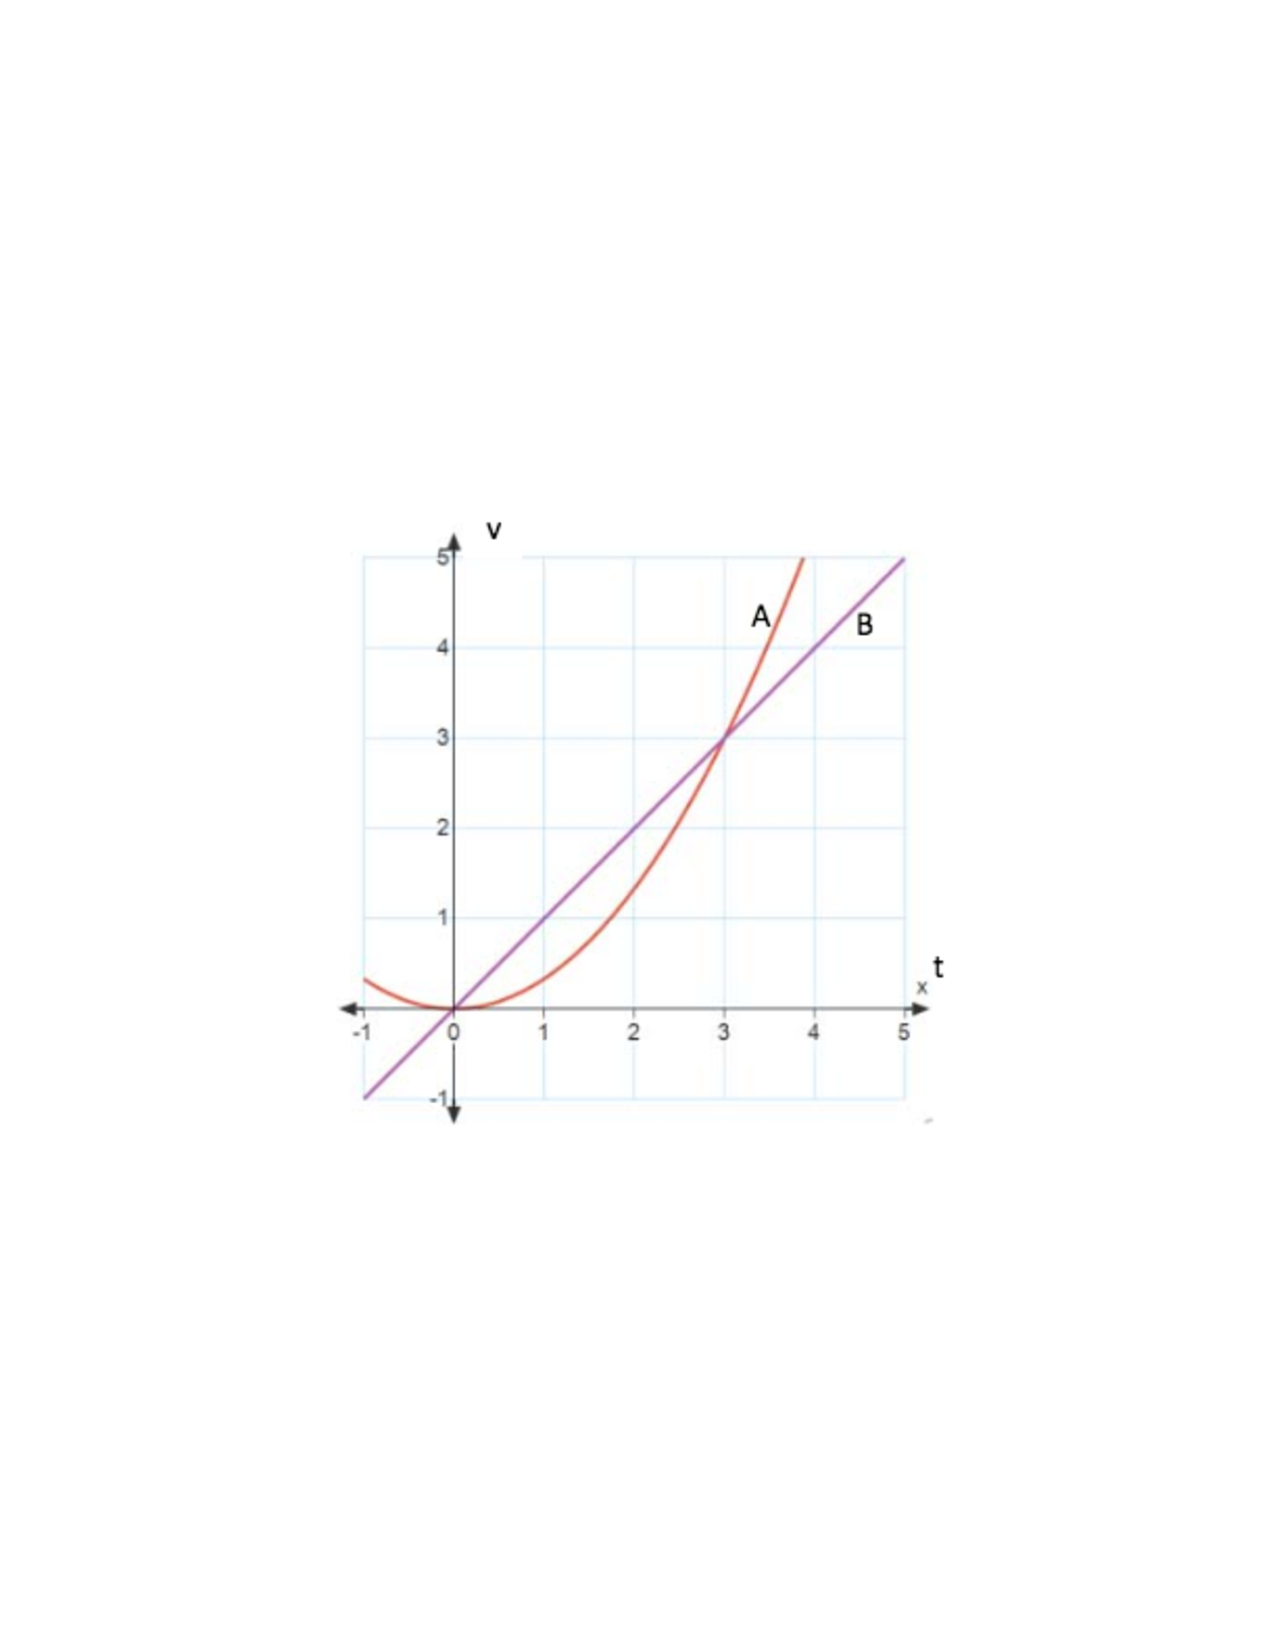
\includegraphics[trim= 270 250 250 250]{Figure6-2-1.pdf}
\end{image}

	\begin{enumerate}
		\item  Who is running the fastest $2$ minutes into the race?
		\begin{freeResponse}
		$v_A(2) = \frac{4}{3}$ and $v_B(2) = 2$.  
		So $B$ is running faster at the $2$ minute mark of the race.
		\end{freeResponse}
		
		\item  Who is winning the race $2$ minutes into the race (and by how much)?
		\begin{freeResponse}
		The distance that $A$ covers in the first $2$ minutes is
		\[
		\int_0^2 v_A(t) \d t = \int_0^2 \frac{1}{3} t^2 \d t = \eval{\frac{1}{9} t^3}_0^2 = \frac{8}{9}.
		\]
		The distance that $B$ covers in the first $2$ minutes is
		\[
		\int_0^2 v_B(t) \d t = \int_0^2 t \d t = \eval{\frac{1}{2} t^2}_0^2 = 2.
		\]
		So $B$ is winning after $2$ minutes.
		
		$B$ is winning by $2 - \frac{8}{9} = \frac{10}{9}$.  
		This could also be calculated by
		\[
		\int_0^2 (v_B(t) - v_A(t)) \d t.
		\]
			\begin{image}
			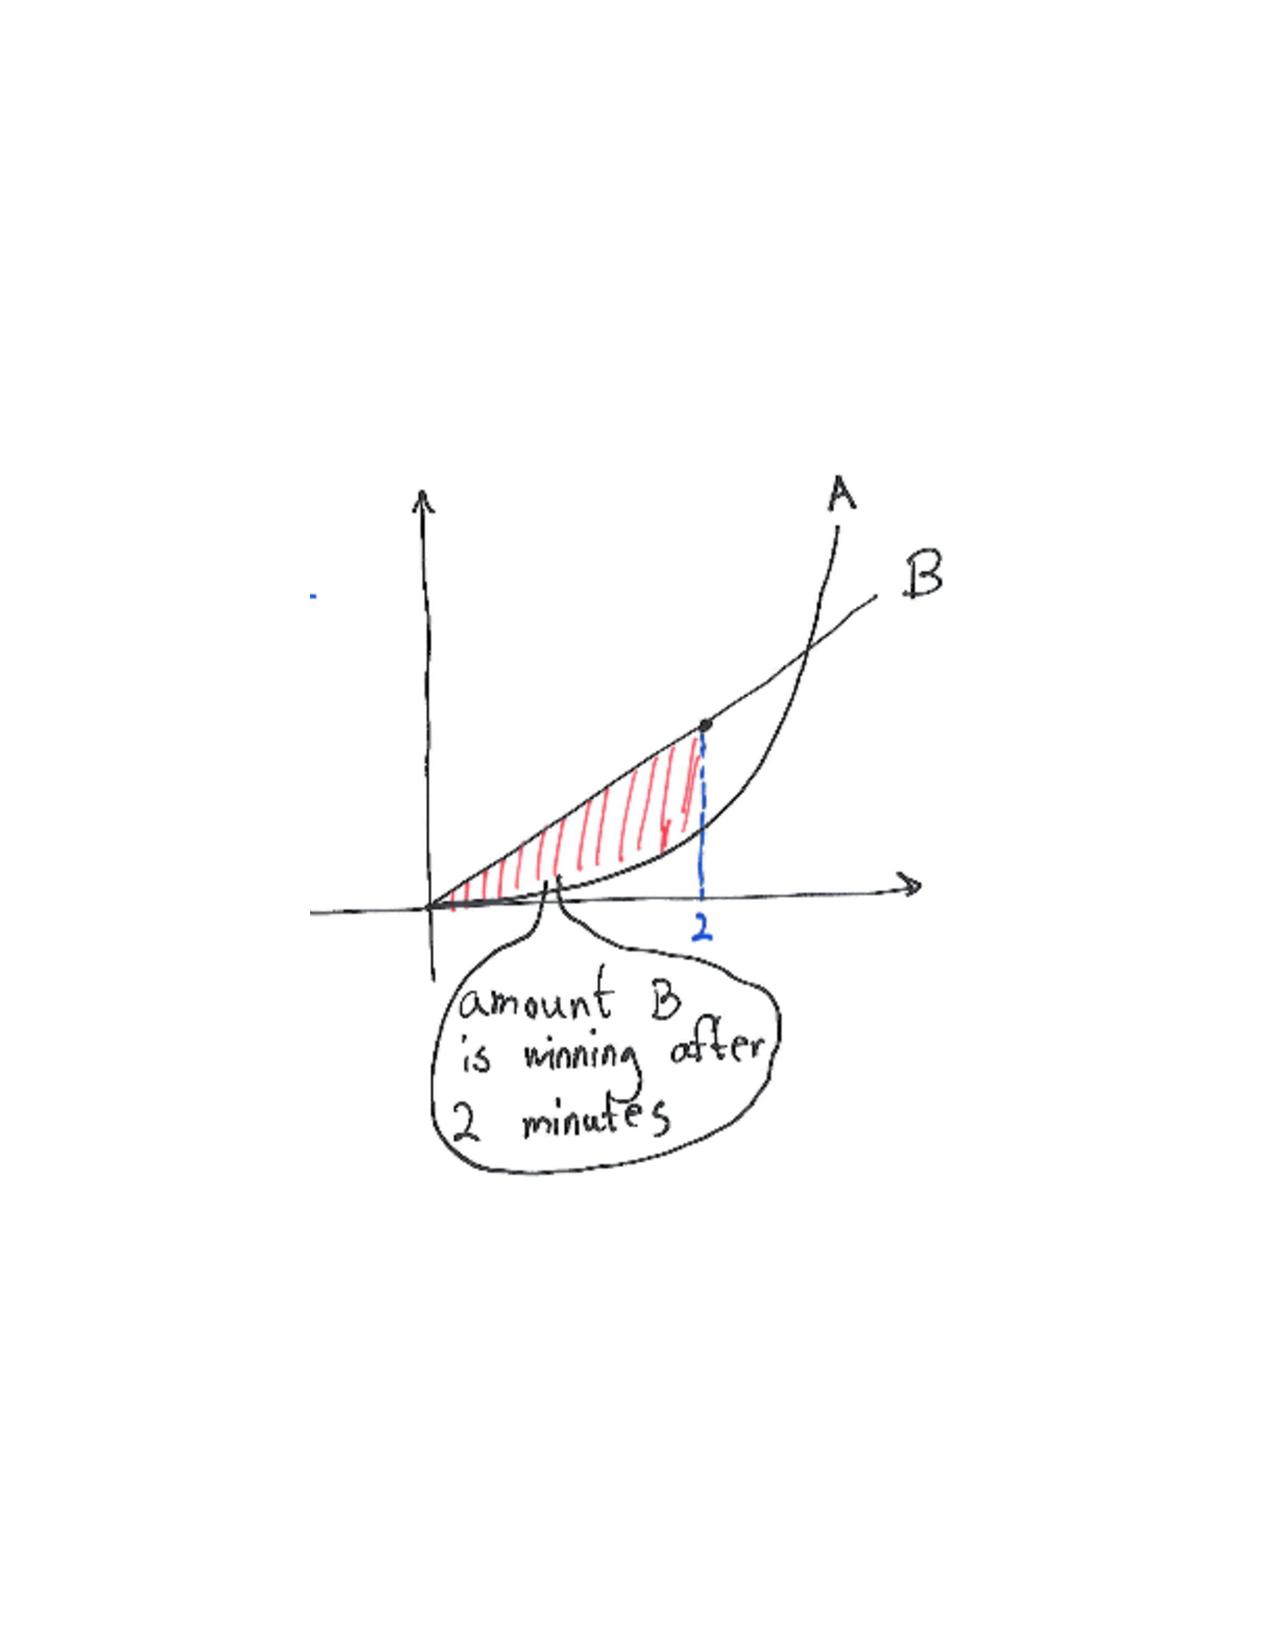
\includegraphics[trim= 130 230 100 230,scale=0.8]{Figure6-2-6.pdf}
			\end{image}
		\end{freeResponse}
		
		\item  What special event occurs $3$ minutes into the race?
		\begin{freeResponse}
		Runner $A$ matches runner $B$'s velocity.  
		ie, $v_A(3) = v_B(3)$.  
		\end{freeResponse}
		
		\item  Who wins the race (and by how much)?
		\begin{freeResponse}
		The distance that $A$ covers is
		\[
		\int_0^4 v_A(t) \d t = \int_0^4 \frac{1}{3} t^2 \d t = \eval{\frac{1}{9} t^3}_0^4 = \frac{64}{9} = 7.\overline{1}.
		\]
		The distance that $B$ covers is
		\[
		\int_0^4 v_B(t) \d t = \int_0^4 t \d t = \eval{\frac{1}{2} t^2}_0^4 = 8.
		\]
		So runner $B$ wins.  The amount that $B$ wins by is
		\[
		8 - \frac{64}{9} = \frac{8}{9}.
		\]
		This could have also been computed by
		\[
		\int_0^4 (v_B(t) - v_A(t)) \d t.
		\]
			\begin{image}
			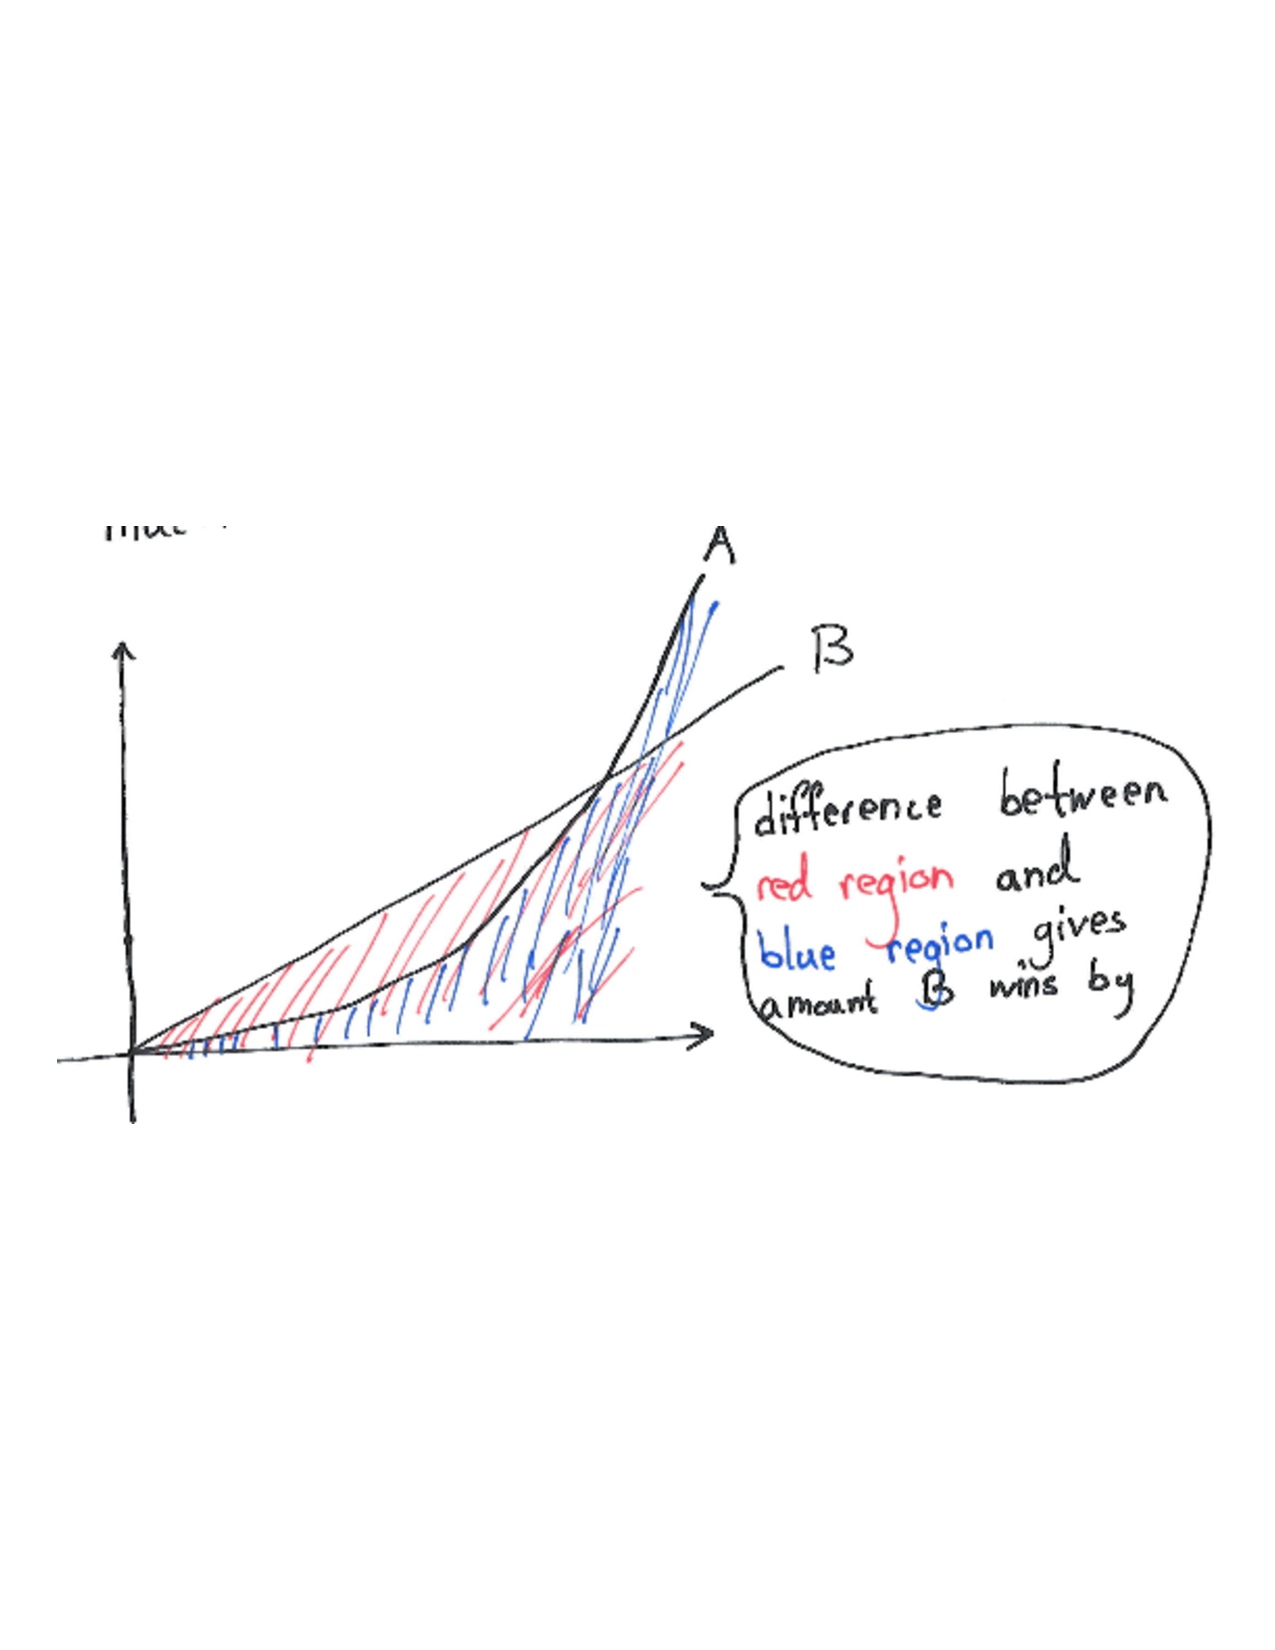
\includegraphics[trim= 130 250 100 250,scale=0.6]{Figure6-2-7.pdf}
			\end{image}
		\end{freeResponse}
		
		\end{enumerate}

\end{problem}

\begin{instructorNotes}
Do this problem as a class discussion.  
The main point is to have students identify how each of the questions relates to the graph of the velocity functions.
\end{instructorNotes}
















	
	
	
	
	
	
	
	
	

	










								
				
				
	














\end{document} 


















